\chapter{Introduction}
\label{c:intro}

% Background

%# of mobile phone users
With the increasing adoption of smartphones~\cite{increasing-phones}, more and more software developers are interested in building mobile applications for smartphones~\cite{attract-game-developer}. Among the various types of mobile applications, game is the most popular. According to \cite{gamepercent1} and \cite{gamepercent2}, by 2010, about 58 percent of the applications in the biggest mobile application store (i.e., Apple's App Store) are games.

However, on Google's Android platform, existing tools for game development are still not perfect. For instance, developers need to deal with the low-level details of JNI (Java Native Interface) calls such as method signature when using Android NDK (Native Development Kit) ; are not able to use GLSL (OpenGL Shading Language) for mathematical computation; and are more difficult to build an application with satisfying performance by using Android SDK (Software Development Kit).

More specifically on the limitation, Java interacts poorly with most current 3D APIs: (1) The interface of Java and native GL is not ideal; (2) Lots of copies or translations needed. Current 2D application performance is not what we would like: (1) Walking through the view hierarchy is slow; (2) Applications need to be called each time we render , e.g., \textit{onDraw()}.; (3) Skia is a poor fit for GL acceleration; (4) We are not in a position to scale to multiple threads; and more importantly, (5) we need 3D apps, Skia performance on larger size screen is unacceptable.

To overcome above limitations, Google introduces a framework, \RS{}\cite{renderscript-part1}, in Android SDK 3.0 named Honeycomb. (For simplification, we use RS and \RS{} interchangably in this thesis.) 

\RS{} aims to provide high performance 3D rendering and mathematical computation at the native level, which targets for the following goals: (listed from most to least important) \cite{renderscript-part2}
\begin{itemize}
	\item \textbf{Portability} ─{} Application code needs to be able to run across all devices with different hardware, and be able to fully utilize the capability of various hardwares. For example, ARM currently comes in several variants: with and without VFP, with and without NEON, and with various register counts. Beyond ARM, application code should be able to run on other CPU architectures such as x86, or even run on a GPU or a DSP.
	\item \textbf{Performance} ─{} The second goal is to get as much performance as possible under the requirement of portability. 	
    \item \textbf{Usability} ─{} The third goal is to simplify development as much as possible by offloading the heavy lifting of interfacing with a native graphics API while retaining full application control. Where possible we automate steps to avoid hand-written glue code and other developer-side busy work.
\end{itemize}

% Propose

There are two kinds of \RS{}s: compute and graphics. A compute \RS{} does not do any graphics rendering while a graphics \RS{} does.

A \RS{} application comprises both Java codes and native codes. Similar to other Android applications, the Java code in a \RS{} application uses Android SDK API. The native code, or the RS script in other words, is actually written in a C99-standard C language with extensions such as vector operations, function overloading, and rsForEach() parallelization. Note that a \RS{} application contains at least one RS script, you write and save it to a .rs file in your project. 
The communication between Java codes and native codes is through JNI function calls. Simply stated, there are \textbf{two layers and one bridge in between}:
\begin{itemize}
\item Android \textit{System Layer} (\textbf{Java Framwork}, i.e., \textit{framework.jar}) : That is, traditional framework APIs, which include the \RS{} APIs in \verb|android.renderscript|. \Client{} handles things such as the Activity lifecycle management of your Android application and communicates with the native \RS{} code via \textit{Bridge}.
\item \textit{Native Layer} (Codes stored in the \textbf{native .rs files}) : \Core{} is responsible for doing intensive computing and graphics rendering tasks. \Core{} returns the result to \Client{} through \Bridge{}. 
\item \textit{Bridge} (\textbf{JNI}, i.e., \textit{librs\_jni.so}, and \textbf{reflected Java classes}) : \Bridge{} deals with the communication between the above two layers. The Android build tools automatically generate the classes for \Bridge{} during the build process. \RS{} uses lockless FIFO (First In and First Out) command queue to communicate between layers. Figure \ref{fig:Java-C-communicate-flow} shows the flow of communication.
\end{itemize}

\begin{center-figure}
    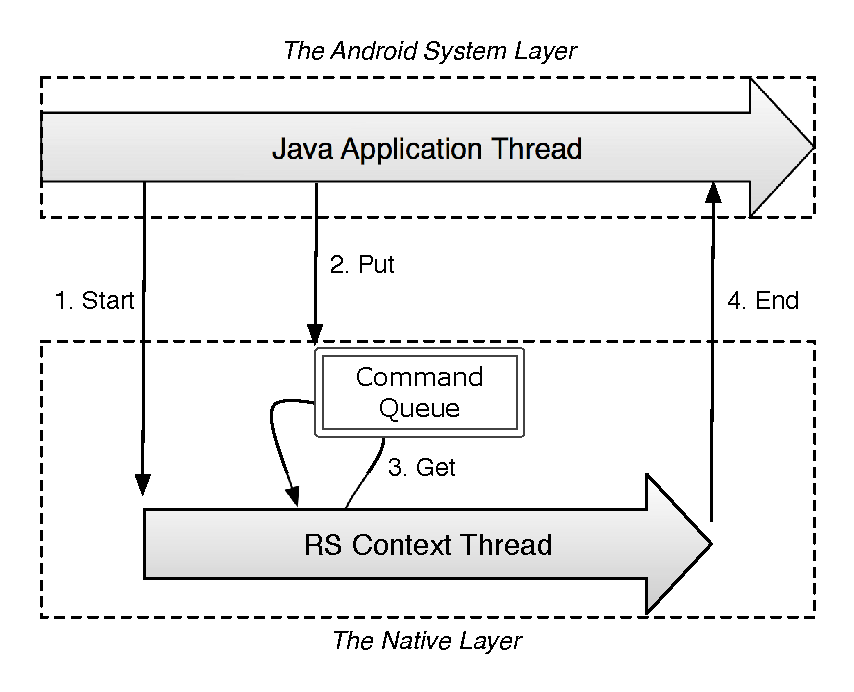
\includegraphics[scale=0.8]{fig/LocklessFifo.eps}
    \caption{Communication between Java and RS code}
    \label{fig:Java-C-communicate-flow}
\end{center-figure}

As Figure \ref{fig:Java-C-communicate-flow} shows, minimal work is done in the application thread, and no native drawing calls are directly from Java application codes. (i.e., All drawing calls are invoked from \Core{}) The RS native thread does heavy lifting: screen can be refreshed without a callback to the Java application thread.

\begin{enumerate}[label=Step \arabic*., font=\sffamily\bfseries]
\item When a \RS{} application is launched, \Client{} creates a Java application thread. After being initialized, the Java application thread notifies \Core{} to create an RS context thread and establish the command queue via \Bridge{}. 
\item Both computing and rendering are done at \Core{} and UI events are handled in the \Client{}. Once the Java application thread receive an event, it puts the commands for computation or rendering into the FIFO command queue.
\item If all of the conditions are met, RS context thread will keep polling the command queue until getting a command. While getting a command, the RS context thread executes the command in \Core{}. (See Chapter \ref{ss:ThreeCondition})
\item As the RS context thread receives a destory signal, the control is handed over to \Client{}.
\end{enumerate}
We will discuss the flow in more details in Chapter \ref{c:OverviewRS}.

Although the \RS{} framework is a major improvement in development of fancy visual effects and other computing intensive application, developers may find it difficult to develop Renderscript applications due to the absence of a debugger or an emulator. Although Google does provide an emulator for Android Honeycomb, it is only starting to support OpenGL ES 2.0, which is required to run \RS{} applications. 

For reducing the complexity of development and debugging, we need a mechanism which can replay and execute \RS{} commands on the remote engine. To accomplish the objective, we propose the \RRS{} architecture in this thesis. The main idea of the \RRS{} architecture consists of two steps. Based on the architecture showed in Figure \ref{fig:Java-C-communicate-flow}, first, we extend \RS{} to make it remote-able. To acheive this, we build a \Transport{} on the top of \Core{}. \Transport{} takes care of sending commands of a local \RS{} system to a remote \RS{} system. Figure \ref{fig:transport-layer} below illustrates that.

\begin{center-figure}
    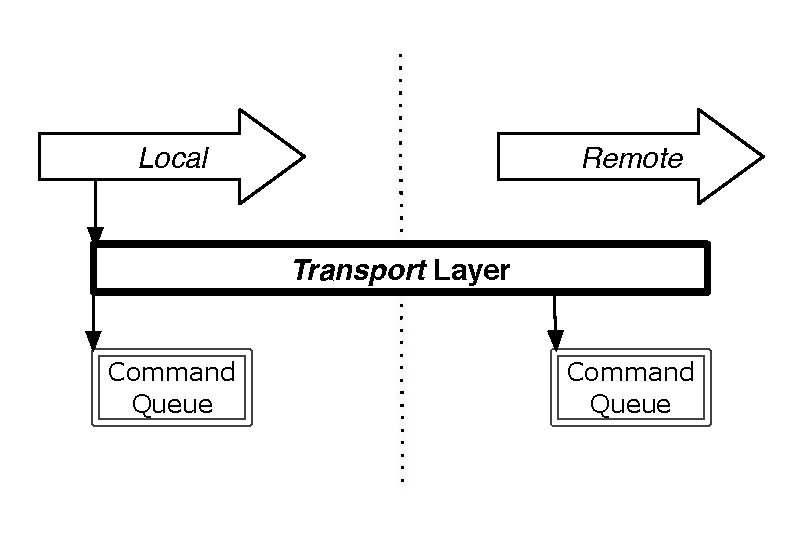
\includegraphics[scale=0.8]{fig/TransportLayer.eps}
    \caption{Transport Layer}
    \label{fig:transport-layer}
\end{center-figure}

Second, we replay the commands on the remote engine by materializing the commands on top of a remote engine. Depending on the type of remote engines, the replay may need to map \RS{} commands to egl, glx, agl, or wgl\footnote{They are OpenGL interfaces for Android, Linux, Mac OS, and Windows, respectively.}. Note that both rendering and computing commands are played in individual engine so that we could leverage the hardwares on the remote engine. The egl-mapped implementation is demonstrated in this thesis.
%Any smart device is just like a personal-cloud. After the authentication, we could do the above ones by sending commands to each other.
With \RRS{}, we could send the commands from emulator and replay it on the remote host. In this scenario, the remote host is local machine. In our implmentaion, extended \RS{} runtime could enable the debugging option by setting the property via ADB (Android Debugging Bridge).

Additionally, \RRS{} has the potential to be the foundation of many other applicaiotns in addition to debugging, such as remote controlling, collaborating tools, multi-player games, remote monitoring, and etc. 

The rest of the paper is organized as follows. Chapter 2 describes related works. As a background knowledge, Chapter 3 goes through the existing design and implementation of \RS{} system. Chapter 4 illustrates our design of \RRS{}. Chapter 5 discusses the egl-mapped implementation for \RRS{}. Finally, Chapter 6 concludes the thesis and presents the future works.
